\documentclass[12pt]{article}    
\usepackage{ucs} 
\usepackage[utf8x]{inputenc}
\usepackage[russian]{babel}  
\usepackage{float}
\usepackage{amsmath}
\usepackage{autonum}
\title{Лабораторная работа №5\\
	Определение удельного заряда электрона}
\author{Хафизов Фанис}
\usepackage[pdftex]{graphicx}
\usepackage{multirow}
\begin{document}
	\begin{figure}
		\centering
		
\includegraphics[width=0.3\linewidth]{logo}
	\end{figure}
	\maketitle
	\newpage
	\section{Цель работы}
	Определить удельный заряд электрона с помощью катушек Гельмгольца.
	\section{Оборудование}
	Узкая электронно-лучевая трубка, катушки Гельмгольца, источник напряжения 300 В, регулируемый источник напряжения 0..300 В, цифровые мультиметры (2 шт), соединительные провода.
	\section{Порядок действий}
	\begin{enumerate}
		\item Соберем экспериментальную установку.
		\item Зафиксируем значение напряжения $U=150$ В и снимем зависимость $r(I)$ радиуса пучка электронов от силы тока в катушках.
		\item Зафиксируем силу тока в катушках равную $I=1,5$ А и снимем зависимость $r(U)$ циклотронного радиуса электронов от ускоряющего напряжения.
	\end{enumerate}
	\section{Теоретическая зависимость}
	\[
	r(I,U)=\frac{R}{\mu_0n}\sqrt{\frac{125}{32\gamma}}\frac{\sqrt{U}}{I}
	\label{eq}
	\]
	Следовательно, зависимости $r(1/I)$ и $r(\sqrt{U})$ линейны.
	\section{Таблицы данных и графики}
	\begin{table}[H]
		\centering
		\begin{tabular}{|l|r|r|}
			\hline
			$r$, см & \multicolumn{1}{l|}{$I$, А} & \multicolumn{1}{l|}{$1/I$, 1/А} \\ \hline
			2,0     & 3,37                        & 0,297                           \\ \hline
			2,5     & 2,67                        & 0,375                           \\ \hline
			3,0     & 2,2                         & 0,455                           \\ \hline
			3,5     & 1,89                        & 0,529                           \\ \hline
			4,0     & 1,62                        & 0,617                           \\ \hline
			4,5     & 1,43                        & 0,699                           \\ \hline
			5,0     & 1,27                        & 0,787                           \\ \hline
		\end{tabular}
		\caption{Зависимости $r(I)$ и $r(1/I)$}
	\end{table}
	\begin{table}[H]
		\centering
		\begin{tabular}{|l|r|r|}
			\hline
			$r$, см & \multicolumn{1}{l|}{$U$, В} & \multicolumn{1}{l|}{$\sqrt{U}$, $\sqrt{B}$} \\ \hline
			2,0     & 49                          & 7,0                                         \\ \hline
			2,5     & 54                          & 7,3                                         \\ \hline
			3,0     & 63                          & 7,9                                         \\ \hline
			3,5     & 90                          & 9,5                                         \\ \hline
			4,0     & 129                         & 11,4                                        \\ \hline
			4,5     & 169                         & 13,0                                        \\ \hline
			5,0     & 218                         & 14,8                                        \\ \hline
		\end{tabular}
		\caption{Зависимости $r(U)$ и $r(\sqrt{U})$}
	\end{table}
	\begin{figure}[H]
		\centering
		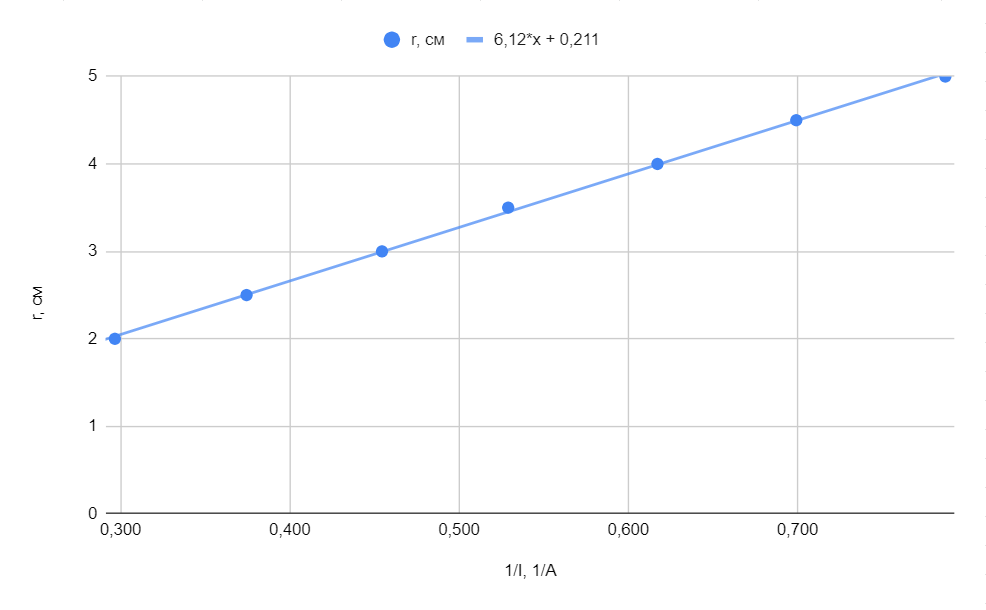
\includegraphics[width=0.9\linewidth]{graph1}
		\caption{График зависимости $r(1/I)$}
	\end{figure}
	\begin{figure}[H]
		\centering
		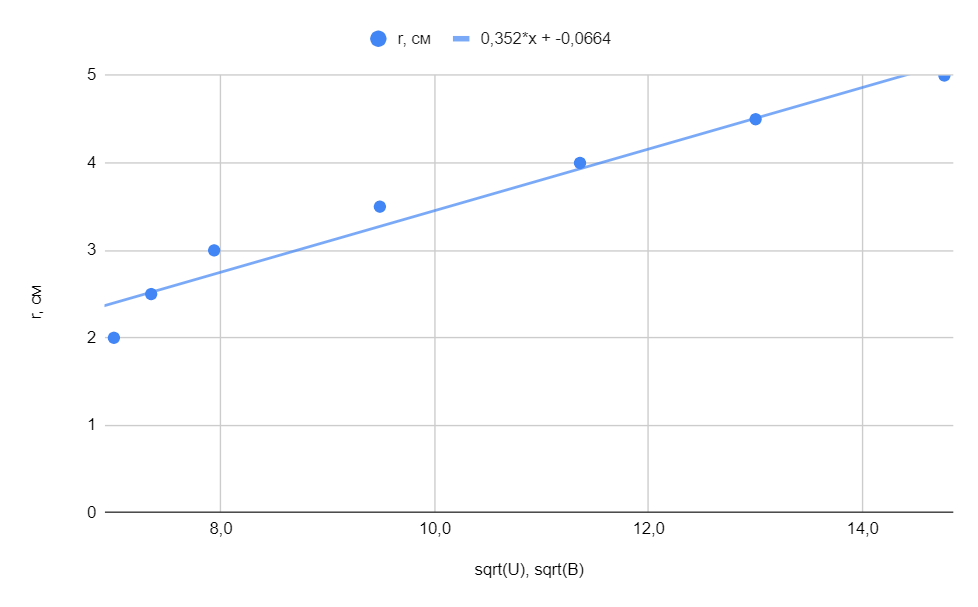
\includegraphics[width=0.9\linewidth]{graph2}
		\caption{График зависимости $r(\sqrt{U})$}
	\end{figure}
	Как можно заметить, в графике зависимости $r(\sqrt{U})$ первые две точки выбиваются из всей серии, что можно объяснить нестабильностью пучка электронов при малых значениях ускоряющего напряжения. Построим этот график без этих двух точек.
	\begin{figure}[H]
		\centering
		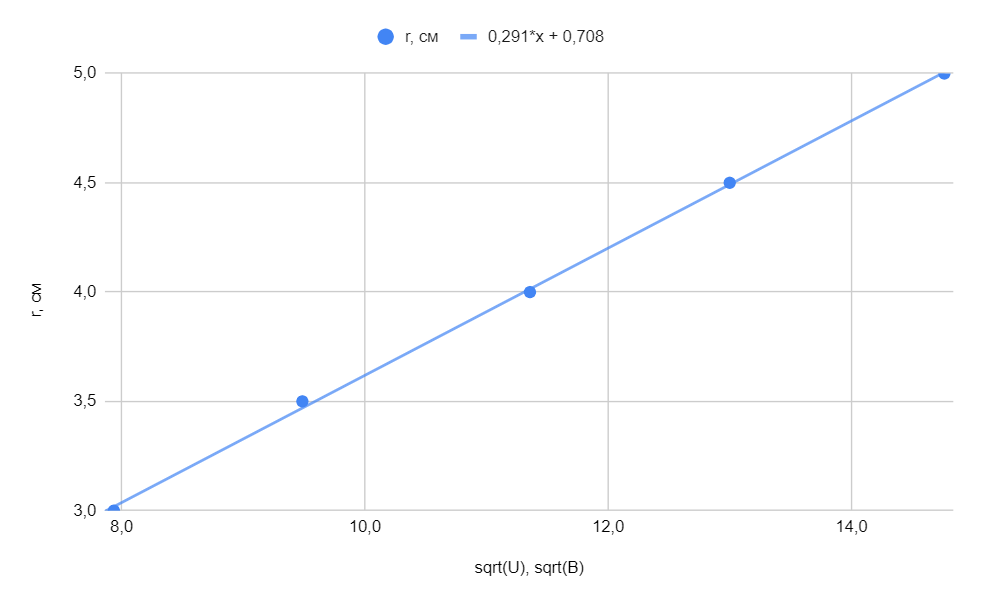
\includegraphics[width=0.9\linewidth]{graph3}
		\caption{График зависимости $r(\sqrt{U})$ без 2 точек}
	\end{figure}
	\section{Расчеты}
	Из коэффициента наклона графика $r(1/I)$:\\
	$\displaystyle\alpha = 6,12$ см$\cdot$А$=6,12\cdot10^{-2}$м$\cdot$А\\
	Из формулы (\ref{eq}):\\
	$\displaystyle\alpha = \frac{R}{\mu_0n}\sqrt{\frac{125}{32\gamma}}\sqrt{U}$\\
	$\displaystyle\gamma=\frac{125}{32}(\frac{R}{\alpha\mu_0n})^2U=\frac{125}{32}(\frac{0,2}{6,12\cdot10^{-2}\cdot1,26\cdot10^{-6}\cdot154})^2\cdot 150=\\=1,66\cdot10^{-11}$Кл/кг
\end{document}
